\section{Theorie}
Die Beugung des Lichts ist ein physikalisches Phänomen, welches sich von der geometrischen Optik differenziert.
Es beschreibt den Vorgang, wie sich Licht in einen geometrisch scheinbar unerreichbaren Raum ausbreitet.
Dies lässt sich auf den Wellencharakter von Licht und dem sich daraus ableitenden huygensschen Prinzip zurückführen.
Das einfachste Beispiel eines Hindernisses ist der Spalt, welcher in diesem Experiment untersucht wird.
Es kann bei der Lichtbeugung zwischen der fresnelschen und der fraunhoferschen Brechung unterschieden werden.
Bei der fresnelschen Anordnung werden interferierende Strahlen unter verschiedenen Winkeln gebeugt.
Das folgt aus der Ursache, dass die Lichtquelle und der Beobachtungspunktes im Endlichen liegen.
Bei der fraunhoferschen Anordnung hingegen lagert die Lichtquelle und der Beobachtungspunkt jeweils im Unendlich, was zur Folge hat, dass parallele Strahlen auf den Spalt treffen.
Außerdem werden interferierende Strahlen im gleichen Winkel gebeugt.
Die beiden Anordnungen und Lichtbeugungen werden in Abbildung \ref{fig:Beugung} dargestellt.

\begin{figure}[H]
    \centering
    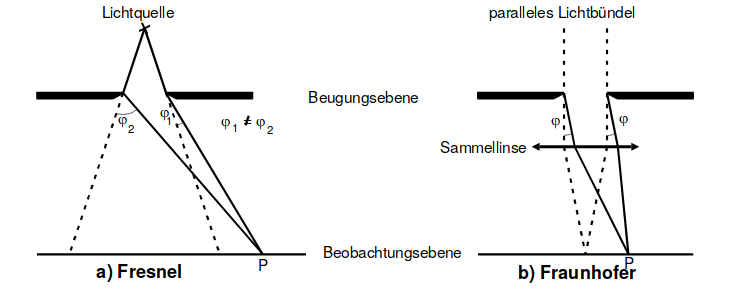
\includegraphics[height=6cm]{Theorie/Beugung.png}
    \caption{Fresnelsche und Fraunhofersche Beugung am Einzelspalt. \cite{1}}
    \label{fig:Beugung}
\end{figure}

Da die fraunhofersche Anordnung mathematisch leichter zu behandeln ist, wird es im Folgenden auch verwendet.
Diese Näherung wird durch einen Laser optimiert.
Es wird ein Spalt verwendet, dessen Länge groß gegenüber seiner Breite $b$ ist.
Der Laser trifft nun mit einer Feldstärke von

\begin{equation}
    A (z,t) = A_0 \; \exp \, \left (\,i \;\left (\omega t - \frac{2 \pi z}{\lambda}\right)\right)
    \label{eqn:Welle}
\end{equation}

auf den Spalt.
Um die Näherung der fraunhoferschen Anordnung zu optimieren, wird der Abstand des Beobachtungspunktes sehr groß zur Spaltbreite gewählt.
Das Interferenzmuster ist mit den Prinzipen nach Fresnel und Huygens zu erklären.
So erzeugt nach Huygens jeder Punkt der Wellenfront im Spalt eine neue kugelförmige Elementarwelle, die nach Fresnel miteinander interferieren.
Um die Interferenz an einem Beobachtungspunkt zu berechnen muss über die gesamte Spaltbreite, also alle Strahlenbündel, summiert werden.
Über den Beugungwinkel $\varphi$ lässt sich nach Abbildung \ref{fig:Einzel} der Gangunterschied auf

\begin{equation}
    \delta = \frac{2 \pi s}{\lambda} = \frac{2 \pi x sin(\varphi)}{\lambda}
    \label{eqn:Gang}
\end{equation}

bestimmen.

\begin{figure}[H]
    \centering
    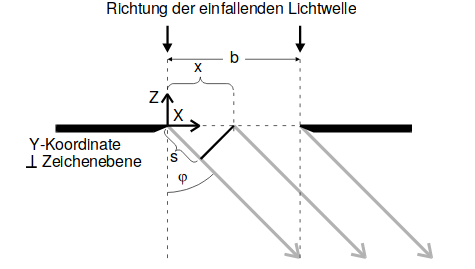
\includegraphics[height=6cm]{Theorie/Einzel.png}
    \caption{Fresnelsche und Fraunhofersche Beugung am Einzelspalt. \cite{1}}
    \label{fig:Einzel}
\end{figure}

Zur Bestimmung der Intensität wird nun zunächst die Amplitudenfunktion in Abhängigkeit des Beugungswinkels bestimmt.
Über Integration und Anwendung der Eulerschen Formel ergibt sich

\begin{equation}
    B(z,t,\varphi) = A_0 \; \exp \, \left (\,i \;\left (\omega t - \frac{2 \pi z}{\lambda}\right)\right) \cdot \exp \, \left (\frac{\pi \; i \; b \; sin(\varphi)}{\lambda} \right) \cdot \frac{\lambda}{\pi \; sin(\varphi)} \cdot sin \left (\frac{\pi \; b\; sin(\varphi)}{\lambda}\right)
    \label{eqn:Amplitude1}
\end{equation}

für die Amplitude.
Die beiden Exponentialanteile von Gleichung \eqref{eqn:Amplitude1} sind für die Messung der Intensiät nicht von Bedeutung.
Das liegt daran, dass die zeitliche und räumliche Abhängigkeit der Amplitude in Ausbreitungsrichtung und der richtungsabhängige Phasenfaktor darauf keinen Einfluss haben.
Somit ergibt sich durch die gegebene Definition für die Amplitude

\begin{equation}
    B (\varphi) = A_0 \; b \; \frac{sin(\eta)}{\eta} \qquad \eta := \frac{\pi \; b \; sin(\varphi)}{\lambda}
    \label{eqn:Amplitude}
\end{equation}.

Aus der Proportionalität der Intensiät zum Amplitudenquadrat ergibt sich für die Intensität

\begin{equation}
    I(\varphi) \propto B(\varphi)^2 = A_0^2 b^2 \left (\frac{\lambda}{\pi \; b \; sin(\varphi)}\right)^2 sin^2 \left(\frac{\pi \; b \; sin(\varphi)}{\lambda}\right)
    \label{eqn:IntEin}
\end{equation}

Die Beugung am Doppelspalt lässt sich nun aufgrund der Überlegung, dass der Doppelspalt eine Überlagerung zweier Einzelspalte ist, analog zur Intensitätsverteilung des Einzelspalts berechnen.

\begin{figure}[H]
    \centering
    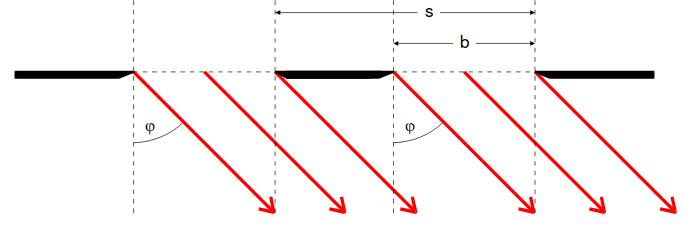
\includegraphics[height=5cm]{Theorie/Doppel.png}
    \caption{Beugung am Doppelspalt. \cite{1}}
    \label{fig:Doppel}
\end{figure}

Mit den Definitionen aus Abbildung \ref{fig:Doppel} und unter der Annahme der fraunhoferschen Lichteinstrahlung, also paralleler Lichtstrahlen, ergibt sich für die Intensitätsverteilung des Doppelspalts

\begin{equation}
    I(\varphi) \propto B(\varphi)^2 = 4 \cdot cos^2 \left(\frac{\pi \; s \; sin(\varphi)}{\lambda}\right) \cdot \left(\frac{\lambda}{\pi \; b \; sin(\varphi)}\right)^2 \cdot sin^2 \left(\frac{\pi \; b \; sin(\varphi)}{\lambda}\right)
    \label{eqn:IntDop}
\end{equation}.

Demnach setzt sich die Intensitätsverteilung für den Doppelspalt aus der des Einzelspalts und einer $cos^2$-Abhängigkeit zusammen.
Außerdem lässt sich die Intensitätsverteilung über die Fourier-Transformierte ausdrücken.
Es ergibt sich mit gegebener Definition

\begin{equation}
    g(\xi) = \frac{2 A_0}{\xi} exp\left(\frac{i \; \xi \; b}{2}\right) sin \left(\frac{\xi \; b}{2}\right) \qquad \xi := \frac{2 \; \pi \; sin(\varphi)}{\lambda}
    \label{eqn:Fourier}
\end{equation}.

Über den Exponentialterm und die Definition von $\xi$ ergibt sich die mathematische Beschreibung des huygensschen Prinzips.